\documentclass[a4paper, 12pt]{article}
\usepackage[utf8]{inputenc}
\usepackage[T1]{fontenc}
\usepackage[english]{babel}
\usepackage{amsmath}
\usepackage{amssymb}
\usepackage{amsfonts}
\usepackage{mathtools}
\usepackage{graphicx}
\usepackage{caption}
\usepackage{subcaption}
\usepackage{float}
\usepackage{wrapfig}
\usepackage{array}
\usepackage{booktabs}
\usepackage{multirow}
\usepackage{colortbl}
\usepackage{xcolor}
\definecolor{darkgreen}{rgb}{0.0, 0.5, 0.0}
\usepackage{geometry}
\usepackage{fancyhdr}
\usepackage[backend=biber,style=apa,sorting=nyt]{biblatex}
\addbibresource{Blanchard.bib}
\geometry{left=1in, right=1in, top=1in, bottom=1in}
\setlength{\headheight}{14.49998pt}
\addtolength{\topmargin}{-2.49998pt}
\usepackage{setspace}
\onehalfspacing
\usepackage{hyperref}
\usepackage{bookmark}
\hypersetup{
    colorlinks=true,
    linkcolor=black,
    citecolor=black,
    urlcolor=black
}
\usepackage{listings}
\usepackage{algorithm}
\usepackage{algpseudocode}
\newcommand{\E}{\mathbb{E}}
\newcommand{\Var}{\mathrm{Var}}
\usepackage{siunitx}
\usepackage{csquotes}
\usepackage{enumitem}
\usepackage{lipsum}

\setlength{\parindent}{1.25cm}
\setlength{\parskip}{0.25cm}

\begin{document}
\pagestyle{fancy}
\fancyhf{}
\lhead{Lucas Dubois}
\rhead{\today}
\cfoot{\thepage}
\renewcommand{\headrulewidth}{0pt}
\begin{titlepage}
\vspace{12cm}
\par
\textit{Master Thesis in Economics with finality Macroeconomics and Finance}
\par
\textit{HEC Liege}
\par
\textit{Supervisor: Malka Guillot}
\par
2024-2025
\begin{center}
\rule{\linewidth}{1pt}
\vspace{0,5cm}
\vspace{0.75cm}
\begin{spacing}{1.75}
{\LARGE \textbf{\textit{Top-Income Inequality in Brazil: The Role of Dividend Taxation}}}
\vspace{0.75cm}
\end{spacing}
\rule{\linewidth}{1pt}
\vspace{0,5cm}
\\
\textbf{{\large Lucas Dubois}}
\\
\vspace{0,5cm}
{(s216283)}\end{center}
\vspace{0.5cm}
\begin{abstract}
    \hspace{1cm} As seen in the course, the New Keynesian (NK) model serves as a fundamental framework in macroeconomic theory and the formulation of monetary policy. 
At its core lies the concept of \textit{divine coincidence}, which suggests that stabilizing inflation successfully stabilizes the output gap that influences welfare. 
This finding significantly eases the challenges faced by central banks since it clearly implies that prioritizing inflation control is enough to reach market efficiency.
However, in their 2007 paper, Blanchard and Galí question this assumption by integrating the notion of \textit{real wage rigidities } in the NK framework. 
Their findings reveal that once we take these frictions into account, the divine coincidence disappears.
\end{abstract}

\vspace{3cm}

\begin{center}
{\Large \today}
\end{center}
\end{titlepage}
\tableofcontents
\newpage

In 1995, Brazil eliminated its dividend taxes, arguing that double taxation of corporate profits hindered growth and distorted capital allocation.
This tax policy, however, helped the consolidation of a very regressive tax system, in which the 85th percentile pays a higher average tax rate than the 99th by 2022 (Figure~\ref{tab:Figure 1}). 
Since then, inequality in Brazil has remained on the rise, confining the 7th most populous nation to a capital concentrating status quo. 
As of 2022, Brazil's Gini index is 53\%, making it the most unequal country in Latin America and among the top 10 globally\footnote{World Bank, 2022}.
Brazil also has the highest wealth concentration worldwide: the top 1\% holds 48.4\% of national wealth\footnote{Global Wealth Report, 2023}.
\par
Several recent studies have attempted to understand the role of taxation on top income inequality. 
Particularly, \cite{berman2024capital} investigate the impact of dividend taxes on top income inequality in Israel, following the 2017 tax cut. 
They find a significant increase in retained earnings among the top 1\%, which is not observed in other income groups.
Similarly, \cite{nallareddy2021corporate} study the effects of corporate taxes on income inequality, finding that corporate tax cuts led to increases in income inequality, a result that is robust across regressions.
Together, those studies provide a strong empirical framework that will serve as the foundation for my research.
\par
Considering the context of Brazil and the existing literature, I would like to dedicate my master’s thesis to understanding the drivers of top-income inequality in Brazil, with a particular focus on the role of dividend taxation in shaping income distribution.
The database provided by \href{https://wid.world/country/brazil/}{WID} offers a wealth of time series indicators related to income distribution and inequality, which will be crucial for my analysis.
In particular, the study by \cite{morgan2025distribution} presents an extensive analysis of the evolution of income, minimum wages, and wealth in Brazil over a 72-year period (\textit{see} Figure~\ref{tab:Figure 2}), by combining data from various official Brazilian agencies and other non-official microdata sources.
Moreover, the authors provide a well-structured use of the raw data they compiled, along with a solid theoretical framework to understand the evolution of income and wealth in Brazil.
\par    
My approach will be the Synthetic Control Method (SCM), which allows for the construction of a synthetic control group that approximates the characteristics of the treated unit.
This method is particularly useful when the number of treated units is small, as is the case for Brazil.
The SCM was formalized in \cite{abadie2003economic} and further developed in \cite{abadie2010synthetic}.
To improve the model’s efficiency, I will include a set of controls that capture the main determinants of income inequality, such as financial development, openness, government spending, and poverty rates, following the work by \cite{afandi2017determinants} and \cite{roine2009long}.
\pagebreak
\par
Furthermore, in order to optimize the model’s performance, I will use Machine Learning techniques to construct the synthetic controls, as described by \cite{araujo2023synthetic}.
This helps create sparse coefficients that identify the most relevant control units.
Similarly, clustering algorithms will be used to group the control units, reducing the dimensionality of the model and improving its efficiency, while allowing for robustness testing of the results.
This process is yet again demonstrated by \cite{abadie2023penalized}, who used penalized regression to estimate the synthetic control weights.

\newpage

\section*{References}

\printbibliography[heading=none]
\newpage

\section*{Appendix}

\begin{figure}[H]
    \centering
    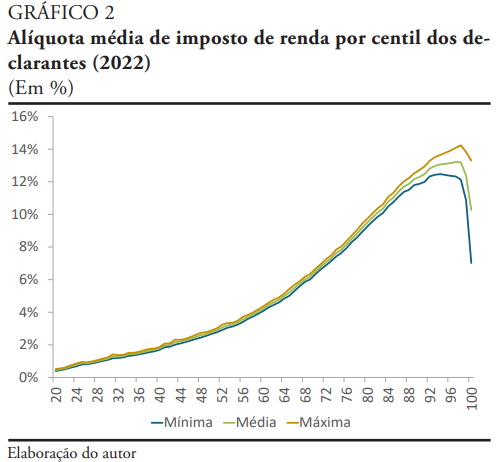
\includegraphics[width=0.6\textwidth]{aliquota.png}
    \caption{Average tax rate by income percentile}
    \label{tab:Figure 1}
\end{figure}

{\Large{\textit{Translation:}}}
\\
\\
Average tax rate by income percentile among reporters (2022).
\\
(As a \%)
\\
\textcolor{blue}{\textbf{---}} Minimum \textcolor{darkgreen}{\textbf{---}} Average \textcolor{orange}{\textbf{---}} Maximum.
\\
Source: IBGE, 2022.
\\
\begin{figure}[H]
    \centering
    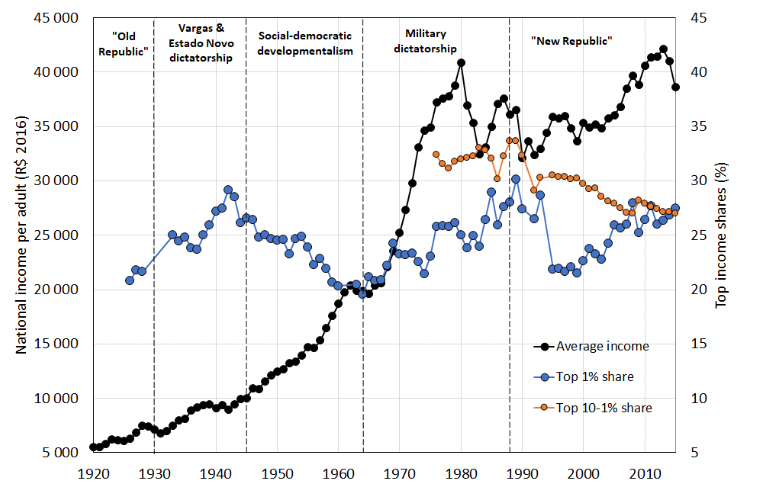
\includegraphics[width=0.6\textwidth]{oneperc.png}
    \caption{Average income over time}
    \label{tab:Figure 2}
\end{figure}

\end{document}